
% 脚の可動班を表示するプログラムの説明

\chapter{脚の可動域を表示するプログラム}\label{chapter:leg_range_python}

\section{概要}
近似的な脚の可動域が適切であるかを評価するためには,
PhantomXの可動域を正確に把握する必要がある.
そのためには可動域の可視化を行うことが必要だろう.
そこで,PhantomXの脚の可動域を可視化するプログラムを作成した.
プログラムは簡単のためPythonを用いて作成しており,
GitHubを通じてだれでも利用できるようにしている.
以下にプログラムの導入方法を説明し,
プログラムの仕様について述べる.

\section{導入方法}
プログラムはGitHubを通じて公開しているため,
まずはGitHubからプログラムをダウンロードする方法を説明する.
そしてPythonのプログラムをコンパイルする方法を説明する.

\subsection{Gitの使用方法}
Gitとは,ソースコードなどの変更履歴を記録・追跡するための分散型バージョン管理システムである.
かみ砕いて言うならば,Googleドキュメントの履歴機能や,
Microsoft Wordの変更履歴機能のようなシステムをさまざまなプログラムのソースコードに対して適用したものといえるだろう.
また,GitHubとは,Gitを用いてソースコードを管理するためのサービスである.
GitHubを用いることで,ソースコードの変更履歴を保存することができるだけでなく,
自分のソースコードを公開したり,他の人が作成したソースコードをダウンロードしたりすることもできる.

\subsubsection{Gitのインストール}
Gitを使うため,まずはGitをインストールする必要がある.
次のリンクからGitのインストーラをダウンロードし,実行する.
インストーラではオプションの設定を変更する必要はないため,
すべてのページで変更をせずに「Next」を選択してインストールを行う.

\begin{itemize}
  \item Git for Windows https://git-scm.com/downloads (アクセス日 2023/12/30)
\end{itemize}

Gitは多くのアプリケーションとは違い,コマンドを用いて操作を行う.
そのため,インストールが完了しても,Gitのアプリケーションが起動することはない.
Gitのインストールが成功したかどうかは,コマンドを用いて確認する.
インストールが完了した場合,Gitのコマンドが使用できるようになっているはずである.
1度パソコンを再起動したのち,\figref{fig:git_bash}のように
スタートメニューに「Git Bash」と入力してGit Bashを起動する.
Git Bashが起動したら,\coderef{lst:git_version}のコマンドを入力する.
\figref{fig:git_version}のようにGitのバージョンが表示されれば,インストールは成功している.
\\
\begin{lstlisting}[caption=Gitのバージョン確認コマンド, label=lst:git_version]
  git --version
\end{lstlisting}

\begin{figure}[h]
  \begin{tabular}{cc}
      \begin{minipage}{.5\textwidth}
          \centering
          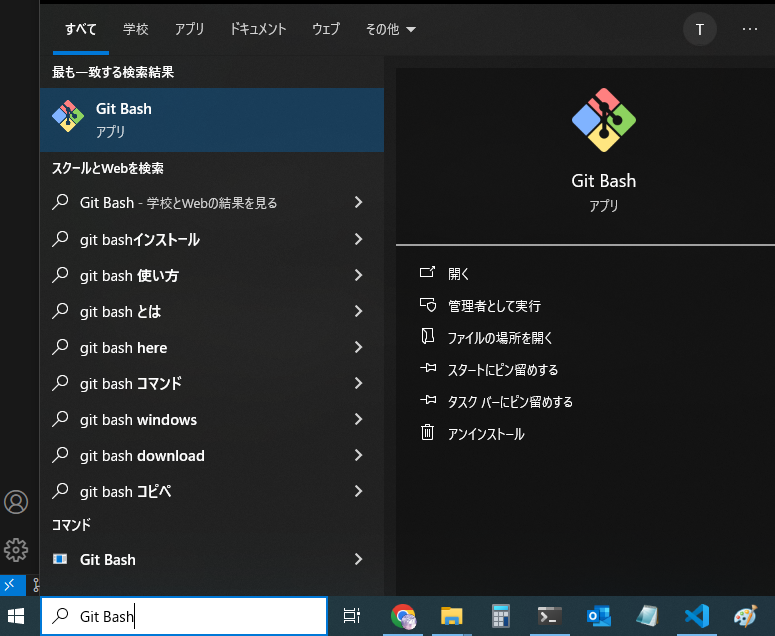
\includegraphics[width=1.0\linewidth]{figure/appendix/git_bash.png}
          \caption{Git Bash}
          \label{fig:git_bash} % chktex 24
      \end{minipage}
      \begin{minipage}{.5\textwidth}
          \centering
          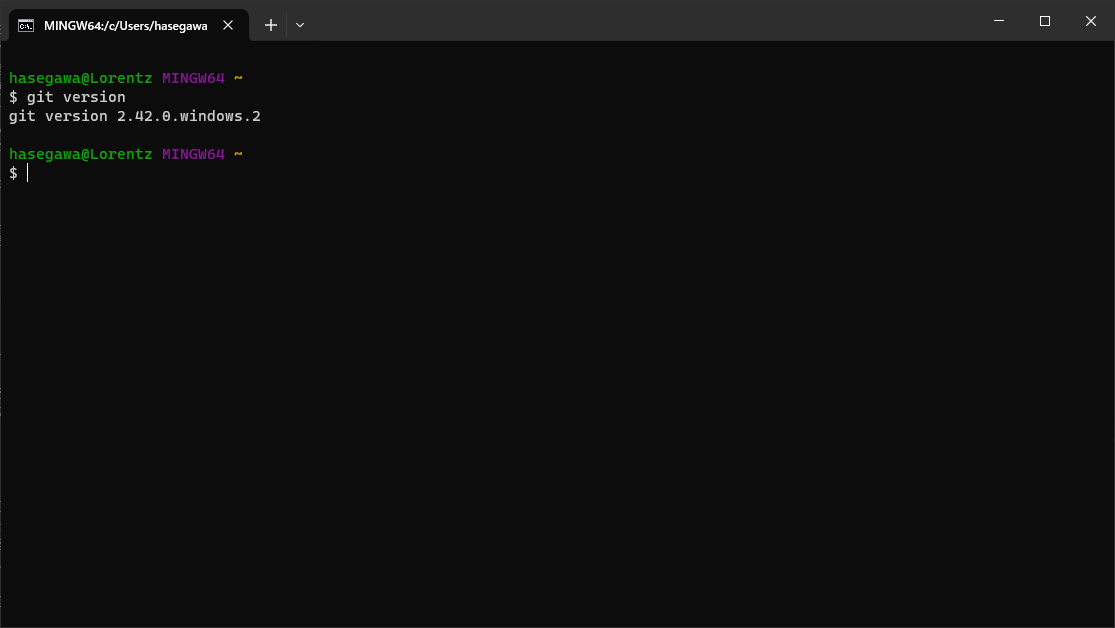
\includegraphics[width=1.0\linewidth]{figure/appendix/git_version.png}
          \caption{Display Git Version}
          \label{fig:git_version} % chktex 24
      \end{minipage}
  \end{tabular}
\end{figure}

\subsubsection{GitHubのアカウント作成}
次にGitHubからプログラムをダウンロードする方法を説明する.
まずはGitHubのアカウントを作成する.
GitHubのアカウントを作成するためには,次のリンクからアクセスし,
アカウント作成の手順にしたがってアカウントを作成する.
アカウントが作成できれば,次のような画面が表示される.


\subsubsection{レポジトリのフォーク,クローン}

\subsection{pythonのコンパイル方法}
本項目では,Windows 10におけるpythonのコンパイル方法を説明する.
Mac OSやLinuxにおけるpythonのコンパイル方法については,ここでは説明しない.
(しかし,「python Mac 環境構築」,「python Linux 環境構築」などで検索すると最適な方法が見つかるだろう.)

\section{プログラムの仕様}

